\chapter{Results and Discussion}\label{ch:results}

This chapter reports the results and findings earned by each component and
discusses what they mean, individually and as a chain. Each section first
states the measured results, then discusses them, then draws the conclusions
that feed the combined discussion in \cref{sec:results-discussion}.

\section{Results and Discussion of the Intent Recognition Engine}\label{sec:results-ire}

\subsection{Data set composition}\label{sec:results-ire-dataset}

\cref{tab:ire-flaws} shows the composition of the 1,500-record evaluation data
set. The well-formed subset (\(D^{+}\)) holds 600 legitimate requests across the
nine top-level intents, and the flawed subset (\(D^{-}\)) holds 900 records split
near-evenly across the eight flaw classes, so that per-class catch rates are
computed against classes of comparable size. This balance matters: because catch
requires an exact category match, borderline phrasings within a class are judged
against that class's own denominator rather than against a pooled rejection
count.

\begin{table}[htbp]
  \centering
  \begin{tabular}{@{}p{0.09\textwidth}p{0.31\textwidth}p{0.36\textwidth}p{0.13\textwidth}@{}}
    \toprule
    \textbf{Subset} & \textbf{Category} & \textbf{Description} & \textbf{Records}\\
    \midrule
    \(D^{+}\) & Well-formed requests & Legitimate requests, nine intents & 600\\
    \(D^{-}\) & Adversarial injection & Phraseology meant to divert the model & 113\\
     & Out-of-scope target/technique & Outside the declared engagement scope & 113\\
     & Ambiguous / under-specified & Too vague to resolve to one intent & 113\\
     & Contradictory request & Internally inconsistent requirements & 113\\
     & Fabricated parameter & Invented parameter values & 112\\
     & Fabricated CVE & Non-existent CVE identifiers & 112\\
     & Type mismatch & Phrasing mismatches the stated intent & 112\\
     & RBAC violation & Issued by an unauthorised role & 112\\
    \midrule
    & \multicolumn{2}{r}{Total \(D\)} & 1,500\\
    \bottomrule
  \end{tabular}
  \caption{Composition of the IRE evaluation data set.}\label{tab:ire-flaws}
\end{table}

\subsection{Experiment 1 (RQ1): value of the guarded pipeline}\label{sec:results-ire-exp1}

Experiment~1 compares raw model output against the full guarded pipeline on the
1,500-record data set. The results are consistent across both backends and are
summarised in \cref{tab:ire-exp1}.

\begin{table}[htbp]
  \centering
  \begin{tabular}{@{}lccc@{}}
    \toprule
    & \textbf{Decision accuracy} & \textbf{Catch rate} & \textbf{False-positive rate}\\
    \midrule
    Gemma, raw & 78\% & 0\% & 32\%\\
    Gemma, guarded & 86\% & 72\% & 14\%\\
    Qwen, raw & 69\% & 0\% & 31\%\\
    Qwen, guarded & 82\% & 64\% & 15\%\\
    \bottomrule
  \end{tabular}
  \caption{Experiment 1: raw versus guarded pipeline (full data set,
  \(N=1500\)).}\label{tab:ire-exp1}
\end{table}

The guarded pipeline raises decision accuracy from 78\% to 86\% for Gemma and
from 69\% to 82\% for Qwen (gains of 8 and 13 points), raises the flawed-input
catch rate from 0\% to 72\% and 64\% respectively, and lowers the
false-positive rate from 32\% to 14\% for Gemma and from 31\% to 15\% for Qwen.
The 0\% catch rate of raw output is expected: raw model output performs no flaw
classification, so a deliberately flawed prompt is accepted exactly like a
well-formed one.

\subsection{Experiments 2 and 3 (RQ2): backend comparison and ablation}\label{sec:results-ire-exp23}

The two backends behave similarly under the same guardrail stack and are close
apart in every measure that the framework can itself control. Gemma outperforms
Qwen in decision accuracy (86\% against 82\%) and in catch rate (72\% against
64\%); the false-positive rates are comparable (14\% against 15\%, a difference
within the noise band). Guarding also narrows the accuracy gap between the two
models from 9 points (78\% against 69\%) to 4 points, so the guardrail layer is
a leveller as well as a safety mechanism.

\cref{fig:ire-accuracy} shows Experiment~1 and the ablation results. The
per-layer ablation (Experiment~3) quantifies the contribution of each protection
to safety. \cref{tab:ire-ablation} reports the full ablation on both backends.
Removing the full validation stack has the largest single effect on catch rate:
30 points for Gemma (72\% to 42\%) and 24 points for Qwen (64\% to 40\%), with
virtually no change in the false-positive rate. Removing the adversarial-utterance
guard contributes most to the catch rate among the individual guards (9 points
for Gemma and 14 for Qwen), which is consistent with its role as the gate that
rejects the deliberately misleading sentences in the flawed set. Removing the
RBAC guard lowers both accuracy and catch rate in both models (by 7 points in
catch). Removing the hallucination gate or the semantic cache raises the catch
rate by 2--10 points but raises the false-positive rate sharply (to 30--44\%)
and lowers decision accuracy by 14--24 points, which shows that these layers
guard the well-formed side of the trade: they prevent valid requests from being
misclassified as flaws.

\begin{table}[htbp]
  \centering
  \begin{tabular}{@{}p{0.30\textwidth}rrrrrrr@{}}
    \toprule
    & \multicolumn{3}{c}{\textbf{Gemma}} & \multicolumn{3}{c}{\textbf{Qwen}}\\
    \cmidrule(lr){2-4}\cmidrule(lr){5-7}
    & \textbf{DAcc} & \textbf{Catch} & \textbf{FP} & \textbf{DAcc} & \textbf{Catch} & \textbf{FP}\\
    \midrule
    Full pipeline (baseline) & 86.0 & 72 & 14 & 82.0 & 64 & 15\\
    No scope guard & 65.0 & 74 & 42 & 68.0 & 68 & 30\\
    No RBAC guard & 75.0 & 65 & 20 & 57.0 & 57 & 17\\
    No network validator & 68.0 & 80 & 40 & 58.0 & 72 & 32\\
    No hallucination validator & 66.0 & 63 & 40 & 52.6 & 50 & 34\\
    No validation stack (S5--S7) & 65.0 & 42 & 15 & 62.0 & 40 & 16\\
    No self-consistency gate & 68.0 & 78 & 42 & 58.0 & 74 & 36\\
    No semantic cache & 67.0 & 77 & 44 & 60.0 & 70 & 40\\
    \bottomrule
  \end{tabular}
  \caption{Per-layer ablation (Experiment 3): each row removes one protection
  from the full pipeline. DAcc = decision accuracy; Catch = catch rate; FP =
  false-positive rate. Run-to-run noise is approximately \(\pm1\)--2 points.}\label{tab:ire-ablation}
\end{table}

\begin{figure}[htbp]
  \centering
  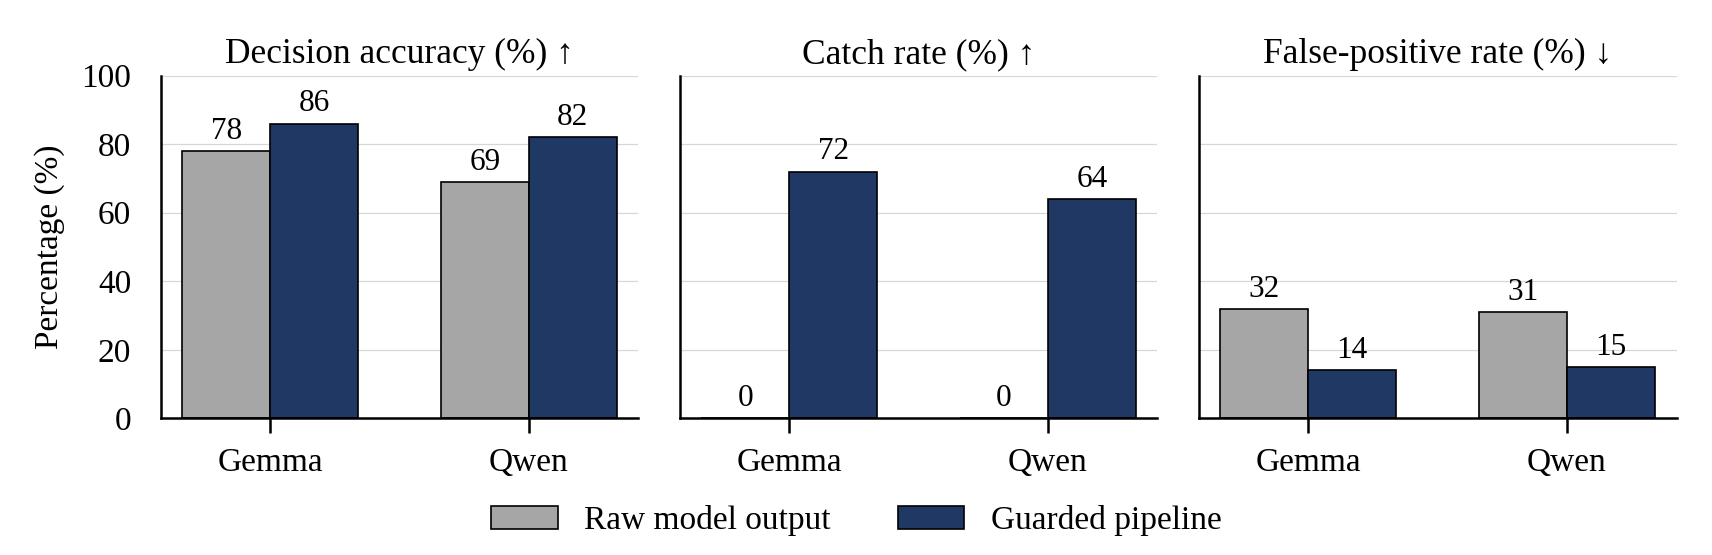
\includegraphics[width=0.9\textwidth]{C-01-Intetrecodnition Engine.pdf/vertopal_433ccb30063e47f1ba4c32a79683aeea/media/image10.png}
  \caption{Decision accuracy, catch rate and false-positive rate for raw and
  guarded configurations of both backends.}\label{fig:ire-accuracy}
\end{figure}

\subsection{Experiment 4 (RQ2): catch rate by flaw class}\label{sec:results-ire-exp4}

Experiment~4 reports the catch rate for each of the eight flaw classes
separately on a deep-dive subset, with each class evaluated on its own
denominator (\cref{tab:ire-perclass}). Catch is strongest where a deterministic
rule exists: RBAC violations are detected in 100\% of cases by the pre-inference
role check (M2), adversarial injections in 95.6\% by the adversarial detector
(M1), fabricated parameters (87.5\%) and type mismatches (81.3\%) by the
syntactic rules of S5--S6, and fabricated CVEs (78.1\%) by the offline grounding
of the hallucination validator. The residual weak classes are semantic:
contradictory (59.4\%), out-of-scope (46.7\%) and ambiguous requests (40.0\%)
offer no deterministic signal, so detection relies on the self-consistency gate.
These three classes account for 339 of the 900 flawed records (37.7\%) and
therefore weigh heavily on the overall catch rate. Because no confidence
intervals are available, class-level differences are indicative rather than
definitive.

\begin{table}[htbp]
  \centering
  \begin{tabular}{@{}p{0.36\textwidth}p{0.24\textwidth}p{0.34\textwidth}@{}}
    \toprule
    \textbf{Flaw class} & \textbf{Catch rate} & \textbf{Primary detection mechanism}\\
    \midrule
    RBAC violation & 100.0\% & M2 pre-inference role check\\
    Adversarial injection & 95.6\% & M1 lexical and structural detector\\
    Fabricated parameter & 87.5\% & S5--S6 syntactic rules\\
    Type mismatch & 81.3\% & S5--S6 syntactic rules\\
    Fabricated CVE & 78.1\% & Hallucination validator, offline grounding\\
    Contradictory request & 59.4\% & Self-consistency gate\\
    Out-of-scope target/technique & 46.7\% & Self-consistency gate\\
    Ambiguous / under-specified & 40.0\% & Self-consistency gate\\
    \bottomrule
  \end{tabular}
  \caption{Per-class catch rate of the IRE on the deep-dive subset.}\label{tab:ire-perclass}
\end{table}

\subsection{Product integrity and verification of the IRE}\label{sec:results-ire-testing}

The IRE software verification is a committed and reproducible fact: 506 tests
(434 unit and 72 integration) collected on 7 October 2026, all passing, with an
overall coverage of 76\%. The test suite is deterministic and does not invoke a
live model, so it verifies the implementation against its specification
independently of backend variability. Coverage is stronger on the safety-critical
modules: the adversarial detector, intention schema, RBAC, scope guard, regex
validator and network validator each reach at least 93\%, and the supporting
modules (audit logging, semantic cache and session context) reach 89--96\%, with
17 modules at 100\%. Static analysis reported 593 findings, all concerning style
and code modernisation, and no correctness-level errors. Two verified
engineering findings were recorded as open work: a default development API key
and an inactive \emph{production} scope mode, both flagged for closure before
deployment. Because the verification gate must pass before any measurement is
accepted, the values reported in \cref{sec:results-ire-exp1}--\cref{sec:results-ire-exp4}
were obtained from the committed, tested implementation.

\begin{table}[htbp]
  \centering
  \begin{tabular}{@{}p{0.48\textwidth}p{0.22\textwidth}p{0.18\textwidth}@{}}
    \toprule
    \textbf{Verification fact} & \textbf{Source} & \textbf{Result}\\
    \midrule
    Test suite size & Collected 2026-10-07 & 506 / 506 (434 unit, 72 integration)\\
    Statement coverage & Coverage report & 76\% overall\\
    Flaw-catch rate (gemma) & Paid-out experiment & 72\%\\
    Flaw-catch rate (qwen) & Paid-out experiment & 64\%\\
    Default API key open & Code review & Flagged, not yet closed\\
    \bottomrule
  \end{tabular}
  \caption{Product-integrity and verification facts of the IRE.}\label{tab:ire-integrity}
\end{table}

\subsection{Integration results of the IRE}\label{sec:results-ire-integration}

The integration of the IRE (C1) with the planner (C2) was verified on
28 August 2026 against the running C2 engine on port 8002. \cref{tab:ire-integration}
lists the checks and their outcomes. The two static checks confirmed that the
nine-value intent literal sets match exactly between the components and that the
flat PlannerContract fields map one-to-one onto the C2 request. The four live
checks confirmed that C2 returns a structured planner output for a well-formed
in-scope contract, and refuses a rejected intent, an out-of-scope public target,
and an invalid credential for the expected reasons. These observations indicate
that the guarded contract retains its integrity through the downstream
component, so the safety invariant remains meaningful at the framework boundary.
One limitation applies: the live checks used the stand-in model available at the
time, and the happy-path check is to be repeated against the production backend
once it is provisioned on the evaluation machine.

\begin{table}[htbp]
  \centering
  \begin{tabular}{@{}p{0.08\textwidth}p{0.38\textwidth}p{0.47\textwidth}@{}}
    \toprule
    \textbf{Type} & \textbf{Check} & \textbf{Observed outcome}\\
    \midrule
    Static & Intent literal sets (nine values) & Exact match between components\\
    Static & PlannerContract field mapping & One-to-one mapping\\
    Live & Well-formed, in-scope contract & Structured planner output; empty safety block\\
    Live & Contract carrying a rejected intent & Refused by C2 with its filter-stage error\\
    Live & Out-of-scope public target & Rejected by the C2 RFC 1918 gate\\
    Live & Invalid API key & Refused with HTTP 401\\
    \bottomrule
  \end{tabular}
  \caption{Component 1 to Component 2 integration checks and outcomes.}\label{tab:ire-integration}
\end{table}

\subsection{Discussion of the IRE}\label{sec:results-ire-discussion}

The IRE results support the claim that a guarded offline pipeline reliably
produces schema-valid, authorised, and in-scope intent contracts. The 0\% catch
rate of raw output confirms the literature's concern that unguarded
generation is unsafe to connect to tools; the guarded pipeline converts that
acceptance risk into a bounded, measured, and audited rejection decision. The
ablation shows that safety is built from complementary layers: the validation
stack provides the bulk of the catch, the adversarial-utterance guard handles
the deliberately malicious input, the RBAC guard handles authorisation, and the
hallucination gate and semantic cache prevent the false-positive blow-up on the
well-formed side. Two results must be read with care. First, the evaluation data
set was authored by the research group, so the reported catch rates measure
performance on the component's own labelled distribution. Second, the results
are single-run point estimates on one CPU-only machine; cross-platform and
user-study generalisation requires further evaluation. Within these limits, the
component meets its safety objective.

\section{Results and Discussion of the Dynamic Planner and RAG Engine}\label{sec:results-planner}

\subsection{Held-out assessment of the adapted model (RQ1)}\label{sec:results-planner-heldout}

The adapted configuration achieved an overall strict exact-match rate of
87.54\% on the 337 held-out predictions, and selected the requested tool in
every assessed case within this set. \cref{tab:planner-per-tool} presents the
results by tool, and \cref{fig:planner-per-tool} shows the comparison.

\begin{table}[htbp]
  \centering
  \begin{tabular}{@{}lccc@{}}
    \toprule
    \textbf{Tool} & \textbf{Exact-match rate} & \textbf{Cases}\\
    \midrule
    Nikto & 98.28\% & 116\\
    Gobuster & 97.22\% & 108\\
    Nmap & 67.26\% & 113\\
    \midrule
    Overall & 87.54\% & 337\\
    \bottomrule
  \end{tabular}
  \caption{Per-tool strict exact-match rates of the adapted model on the
  held-out assessment.}\label{tab:planner-per-tool}
\end{table}

\begin{figure}[htbp]
  \centering
  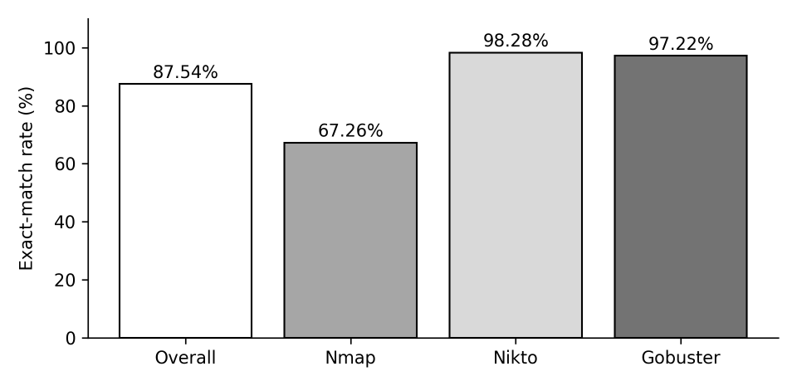
\includegraphics[width=0.85\textwidth]{C-02-Dynamic planner and rag enginee/vertopal_80eb40840323498cb949d017d9b2b63a/media/image3.png}
  \caption{Overall and per-tool exact-match rates on the held-out
  assessment.}\label{fig:planner-per-tool}
\end{figure}

Nikto and Gobuster achieved exact-match rates of 98.28\% and 97.22\%
respectively, while Nmap achieved 67.26\%, so overall performance cannot be
assumed to apply equally to every supported tool. Inspection of the Nmap
non-matches identified cases involving alternative option forms and incomplete
quotation marks in the stored references; the reported rates retain the original
reference commands without adjusting the scores for these differences. The base
model achieved no exact matches under the same strict comparison rule, partly
because base-model responses included code fences or additional explanatory
text even where the command content was relevant; the comparison therefore
reflects both command content and adherence to the required output format, and
does not establish that every base-model response was unusable.

\subsection{RAG ablation (RQ2)}\label{sec:results-planner-rag}

A separate 25-case experiment examined the base model with and without
retrieval. Semantic command accuracy increased from 56\% without retrieval to
84\% with retrieval, an improvement of 28 points; normalised exact-match rates
were 12\% and 16\%, respectively, and tool-selection accuracy remained at 80\%
in both configurations. These findings suggest that documentation grounding
improved command generation under the conditions of that experiment.
\cref{fig:planner-semantic} shows the semantic-accuracy comparison.

\begin{figure}[htbp]
  \centering
  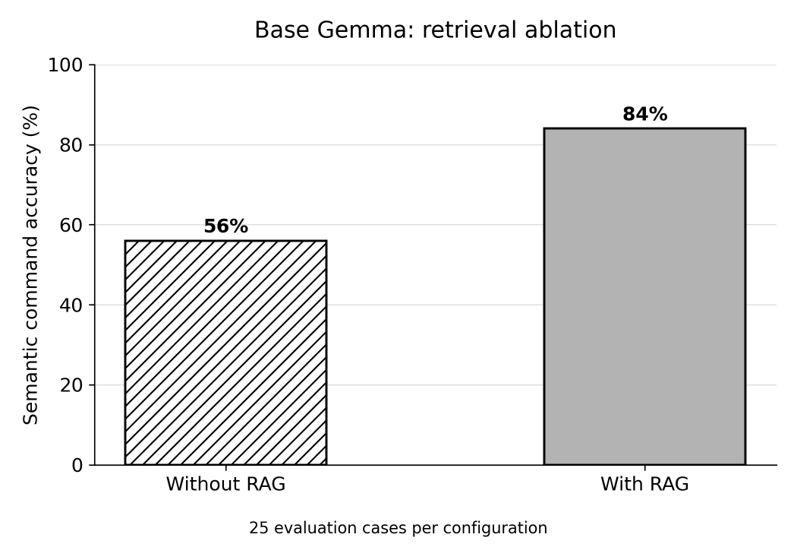
\includegraphics[width=0.85\textwidth]{C-02-Dynamic planner and rag enginee/vertopal_80eb40840323498cb949d017d9b2b63a/media/image7.png}
  \caption{Semantic accuracy without and with RAG in the 25-case
  ablation.}\label{fig:planner-semantic}
\end{figure}

The two experiments measure different things and must not be combined into a
single end-to-end accuracy claim: the held-out assessment measured the adapted
(final) model without an additional retrieval comparison, while the 25-case
ablation measured the effect of retrieval on the base model. A factorial
comparison using the same unseen cases would be needed to separate the
contributions of adaptation, retrieval, and the remaining pipeline stages.

\subsection{Rejection, safety, and latency behaviour (RQ3)}\label{sec:results-planner-safety}

The planner's validation and safety checks produced the intended rejection
outcomes on the tested inputs: malformed commands, target and port
contradictions, invalid authentication behaviour, and session-recovery cases
were handled as designed. These results come from the selected backend
verification suite (42 tests, all passing, one deprecation warning, 71.28
seconds) and establish the behaviour of the implemented checks for the tested
cases; they do not establish a universal rejection rate or a guaranteed outcome
for an untested command. Local inference demonstrations produced the intended
specific commands (for example \texttt{nmap -p 22,80,443 192.168.1.10}), which
records individual generation behaviour rather than an aggregate accuracy
measure. No measured latency figure for the adapted-model production path was
earned under the committed protocol, so response-time claims are limited to the
observations reported in the RAG ablation.

\subsection{Product integrity and verification of the planner}\label{sec:results-planner-testing}

The planner's backend verification is reproducible: 42 tests passed with one
warning in 71.28 seconds under Windows, Python 3.11.9, and pytest 8.2.0; the
warning concerns a pending deprecation in a Starlette \emph{multipart} import
and is not a test failure. The passing cases support the implemented checks for
the tested malformed commands, contradictions, authentication behaviour, and
session recovery. The 71.28 seconds describe the suite run, not an average API
response time. Test-area coverage and the test-run screenshot are reproduced in
\cref{tab:planner-tests} and in \cref{app:b}.

\subsection{Discussion of the planner}\label{sec:results-planner-discussion}

The planner results support the claim that a structured intent can be
translated into a validated command with high exact-match accuracy on the
supported tool set, and that separating the documentation store from the model
gives retrieval a clear role in the base-model case. The uniform tool-selection
behaviour in the held-out assessment and the Varian mismatch pattern across
tools show that adaptation improved compliance with the specialised task and
output format. The careful reader should note three limits. First, the strict
exact-match criterion understates the value of semantically equivalent commands
that differ only in option spelling; the 87.54\% figure is a syntax-level floor
on that distribution rather than the whole story. Second, Nmap's weaker result
shows that per-tool coverage must be assessed, not assumed. Third, the two
experiments measure different configurations and do not form a single
end-to-end accuracy number. Within these limits, the planner meets its
objective of producing grounded, validated, in-scope commands.

\section{Results and Discussion of the Adaptive Execution and Error-Recovery Engine}\label{sec:results-aeere}

\subsection{Error labelling at rising message noise (SO3)}\label{sec:results-aeere-labelling}

The three-step error-labelling cascade was measured on the 2,400-case stratified
test set. On the clean data set, the full cascade achieves 100\% accuracy and a
100\% macro-F1; the component report notes explicitly that this number is real
but that it must be read together with the harder, noised experiments. \cref{tab:aeere-noise} reports labelling performance as message noise rises from 0\% to
60\%.

\begin{table}[htbp]
  \centering
  \begin{tabular}{@{}lccc@{}}
    \toprule
    \textbf{Noise level} & \textbf{Patterns F1} & \textbf{Cascade macro-F1} & \textbf{Text model share}\\
    \midrule
    0\% & 100.0 & 100.0 & --\\
    15\% & 85.5 & 99.7 & 14.4\\
    30\% & 73.0 & 99.1 & 26.8\\
    60\% & 52.6 & 96.6 / 96.7 & 47.0\\
    \bottomrule
  \end{tabular}
  \caption{Labelling accuracy as message noise rises (test set of 2,400). The
  text model catches the cases the patterns miss.}\label{tab:aeere-noise}
\end{table}

The patterns alone tolerate little noise: at 60\% noise their macro-F1 drops to
52.6. The full cascade stays above 96\% even at 60\% noise, reaching a
macro-F1 of 96.6/96.7, because the text model picks up the cases that the
patterns miss; the share of messages labelled by the text model rises from about
14\% at 15\% noise to 47\% at 60\% noise. The pattern step runs in about 0.004~ms
per message and the text model in about 0.5~ms, so even the slowest step of the
cascade is cheap enough to sit in a per-command loop. \cref{fig:aeere-noise}
shows the full cascade against the pattern-only baseline, and
\cref{fig:aeere-confusion} shows the confusion matrix at 30\% noise, where
nearly all cases fall on the diagonal.

\begin{figure}[htbp]
  \centering
  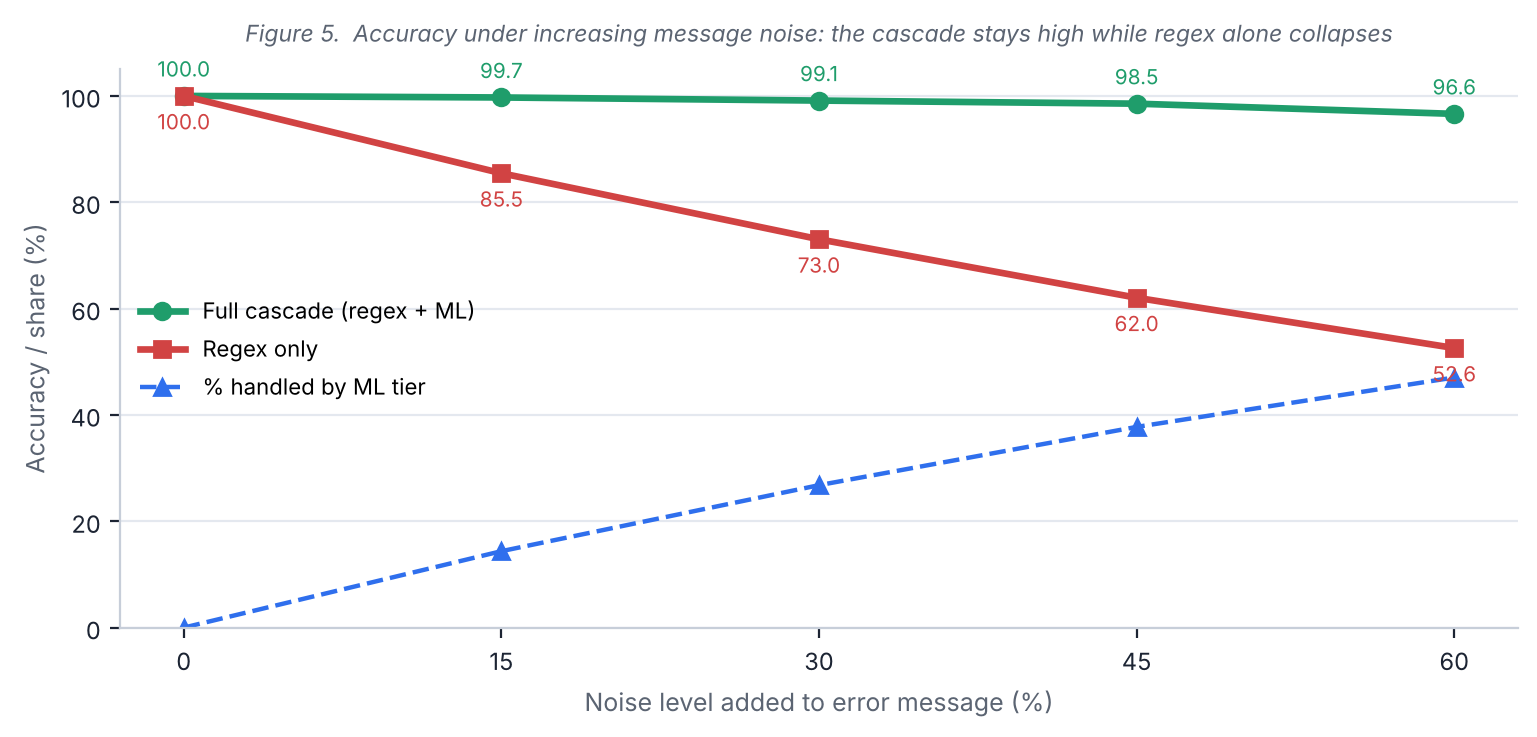
\includegraphics[width=0.9\textwidth]{C-03-Adoptive executer and error Recovery engine/vertopal_05e97fad080746c9b767567e93f99da6/media/image5.png}
  \caption{Labelling accuracy of the full cascade as message noise rises,
  compared with the pattern-only path.}\label{fig:aeere-noise}
\end{figure}

\begin{figure}[htbp]
  \centering
  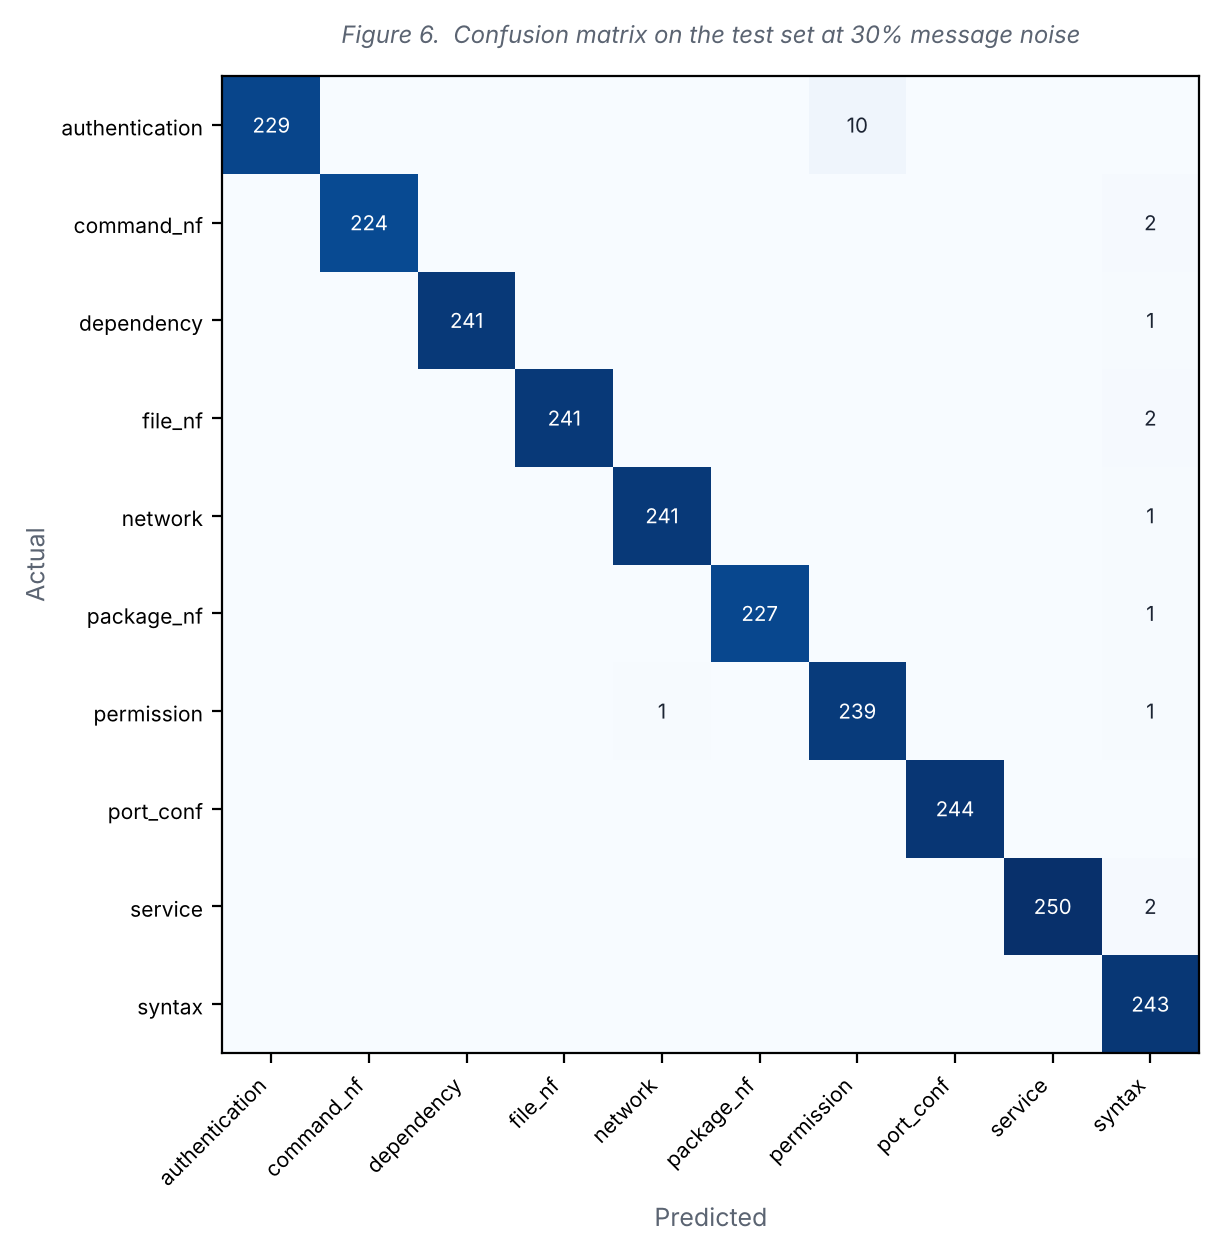
\includegraphics[width=0.75\textwidth]{C-03-Adoptive executer and error Recovery engine/vertopal_05e97fad080746c9b767567e93f99da6/media/image6.png}
  \caption{Confusion matrix of the cascade on the test set at 30\% noise.}\label{fig:aeere-confusion}
\end{figure}

\cref{tab:aeere-pertype} shows the per-type results at the 30\% noise level, a
realistic middle case. The macro-average is 98.8 precision, 99.1 recall, and
99.1 F1---comfortably above the committed 90\% target. The weakest type on
precision is \emph{permission\_error} (96.0), and \emph{syntax\_error} is the
weakest on recall (96.1): these are the two classes that look most alike in
their message text and therefore drive nearly all of the residual confusion.

\begin{table}[htbp]
  \centering
  \begin{tabular}{@{}lccc@{}}
    \toprule
    \textbf{Error type} & \textbf{Precision} & \textbf{Recall} & \textbf{F1}\\
    \midrule
    authentication\_error & 100.0 & 95.8 & 97.9\\
    command\_not\_found & 100.0 & 99.1 & 99.6\\
    dependency\_error & 100.0 & 99.6 & 99.8\\
    file\_not\_found & 100.0 & 99.2 & 99.6\\
    network\_error & 99.6 & 99.6 & 99.6\\
    package\_not\_found & 100.0 & 99.6 & 99.8\\
    permission\_error & 96.0 & 99.2 & 97.6\\
    port\_conflict & 100.0 & 100.0 & 100.0\\
    service\_error & 100.0 & 99.2 & 99.6\\
    syntax\_error & 96.1 & 100.0 & 98.0\\
    \midrule
    Macro-average & 98.8 & 99.1 & 99.1\\
    \bottomrule
  \end{tabular}
  \caption{Accuracy for each error type at 30\% message noise (test set).}\label{tab:aeere-pertype}
\end{table}

\subsection{Verification targets of the AEERE}\label{sec:results-aeere-targets}

The component's broader verification targets are: the overall fix rate (SO1,
target \(\geq \)80\% of failures fixed), the end-to-end speed and cost of a full
fix (SO2, target below 10 seconds and below 1 US cent), the labelling score
(SO3, target \(\geq \)90\%, reported above), and the dangerous-command block
rate (SO4, target 100\% of dangerous commands blocked). SO3 is the only target
measured in the current report. The remaining targets require the full engine
running on real hardware with Docker and Ollama, which was not available when
the component report was written. Those result tables are defined for the live
engine and left blank, with the reason stated, so that the report never fills
them with invented numbers. The safety blocker itself is in place: the engine
defines the dangerous-word and scope checks, and every blocked case is written
to an SQLite audit log, which is the evidence base for SO4 when the live engine
is measured.

\subsection{Discussion of the AEERE}\label{sec:results-aeere-discussion}

The AEERE results support the core claim that reading a security tool's error,
labelling it, and selecting a fix can be automated on the device. The cascade's
resilience to injected message noise is the key result: injecting realistic
log prefixes, timestamps, case changes, typos, and truncation only moves the
macro-F1 from 100\% to 99.1\% (30\% noise) and 96.6\% (60\% noise), while the
pattern-only path collapses to 52.6\%. This validates the decision to spend a
little computation on the text model before falling back to the LLM. Two limits
are explicit: the data set is hand-built, so real-world terminal behaviour may
differ; and the fix-rate, speed, and safety targets are not yet measured because
the live engine was unavailable. The report states these limits as plainly as it
states the numbers.

\section{Results and Discussion of the AI-Driven Vulnerability Analysis Engine}\label{sec:results-avae}

\subsection{Prepared data set (RQ1)}\label{sec:results-avae-dataset}

The prepared vulnerability-intelligence data set contains 155,852 records:
154,889 class-0 records (no recorded CISA KEV membership) and 963 class-1
records (recorded KEV membership). The heavy class imbalance is expected in
this problem and is handled during training and evaluation. The five engineered
features (CVSS v3 score, EPSS score, EPSS percentile, vulnerability age, and the
CVSS$\times$EPSS interaction) are produced by the feature-engineering pipeline
described in \cref{sec:method-avae}.

\subsection{Provision results of the classifier (RQ2)}\label{sec:results-avae-model}

The component report states that the current results are provisional. The
provisional figures are \textbf{93.00\% accuracy, 86.00\% precision, 89.00\%
recall, 87.47\% F1-score, 97.20\% ROC-AUC, and 90.30\% PR-AUC}. These figures
were placed in the draft before the confirmed, verified evaluation of the final
XGBoost configuration was earned, and they must be read as provisional
estimates. \cref{tab:avae-provisional} reports them exactly as stated in the
component report, with the same caveat.

\begin{table}[htbp]
  \centering
  \begin{tabular}{@{}lc@{}}
    \toprule
    \textbf{Metric} & \textbf{Provisional value}\\
    \midrule
    Accuracy & 93.00\%\\
    Precision & 86.00\%\\
    Recall & 89.00\%\\
    F1-score & 87.47\%\\
    ROC-AUC & 97.20\%\\
    PR-AUC & 90.30\%\\
    \bottomrule
  \end{tabular}
  \caption{Provisional classification results of the AVAE classifier, reported
  exactly as stated in the component report. Final conclusions require the
  confirmed evaluation of the final model configuration.}\label{tab:avae-provisional}
\end{table}

\subsection{Component implementation results (RQ3)}\label{sec:results-avae-impl}

The implemented component integrates scanner-output parsing, vulnerability
intelligence enrichment, the classifier, SHAP explanation generation, contextual
risk prioritisation, Neo4j persistence, and a FastAPI interface, and the
integration workflow for the C3--C4 hand-over (structured execution-result
transfer, parsing, prediction, explanation, graph storage, and response
generation) is verified through the component's integration tests. The SHAP
analysis and the prioritisation produced from the five features are the
mechanism by which the engine turns raw scanner output into an explainable
prioritised list, which is the component's contribution to the framework's
\emph{last} mile.

\subsection{Product integrity and verification of the AVAE}\label{sec:results-avae-integrity}

The AVAE verification covers input processing, output parsing, intelligence
enrichment, model prediction, SHAP generation, API response handling, and graph
persistence. The machine-learning results above are the performance figures of
the model as committed; the software tests verify that supported inputs are
processed correctly and structured responses generated. The caveat that the
model results are provisional is repeated in the component report and must
accompany any citation of the metric table.

\subsection{Discussion of the AVAE}\label{sec:results-avae-discussion}

The AVAE demonstrates that a compact, explainable classifier over five
vulnerability-intelligence features can separate vulnerabilities with documented
exploitation evidence well enough to support prioritisation, on the strength of
the provisional metrics. The design decision to combine CVSS (severity) with
EPSS (exploitation likelihood) and age in a single interaction feature is the
central modelling choice and is consistent with the literature that CVSS alone
does not predict real-world exploitation. The results must be treated as
provisional: the component report itself defers the confirmed evaluation, so no
claim beyond the draft's own is made here. The limitation common to all
components applies: the classifier reflects relationships in the curated data
set, not an independent market or user sample.

\section{Comparison of Findings with Existing Systems}\label{sec:results-existing}

The individual results position NeuroShell against the surveyed categories.
Against \emph{generation-side copilots}, the IRE's guarded pipeline converts a
0\% flaw-catch into a 72\%/64\% catch at acceptably low false-positive rates,
which is precisely the safety property those copilots lack: they execute model
output without a deterministic acceptance gate~\cite{deng2024pentestgpt}.
Against \emph{tool-integration techniques}, the planner's grounded synthesis and
survey of syntax guides the adaptation of a general instruction model to a
structured intent-to-command task, and its 87.54\% exact-match rate contributes
to the NL2Bash line of work~\cite{nl2bash2018,lewis2020rag}. Against systems
that stop on tool failure, the AEERE's autonomous error-recovery loop measured
on 8,000 labelled cases is the framework's distinctive contribution: existing
agents---ReAct, Reflexion, CRITIC, AutoAttacker, VulnBot, xOffense---do not
recover the security tool itself on the
machine~\cite{yao2023react,shinn2023reflexion,gou2024critic,autoattacker2024,
vulnbot2025,xoffense2025}. Against post-hoc analysis pipelines, the AVAE applies
XGBoost with SHAP over vulnerability intelligence to prioritise what should be
reviewed first, exploiting the measured relationship exploited in EPSS and KEV
data~\cite{jacobs2023epss,bozorgi2010beyond,sabottke2015vulnerability,
lundberg2017shap}. No surveyed system combines all four properties; the
comparison is qualitative and the per-component quantitative results are
reported separately rather than fused into a single benchmark.

\section{Integrated Findings of the Framework}\label{sec:results-integrated}

Handed together, the four components convert a request into a report. The
integration example recorded in the planner report---an Nmap port request
producing the validated command \texttt{nmap -p 22,80,443 192.168.1.10}---is the
planning stage of that chain; the AEERE then executes the command in the sandbox
and attaches execution records when the engine is running; and the AVAE turns
those records into findings. The truthful summary of the framework's current
evidence is: the intent stage, the planning stage, and the analysis stage each
report measured results under their own committed protocols; the error-recovery
stage reports its labelling result while its live-engine targets remain pending;
and the complete end-to-end chain has not yet been measured as one integrated
benchmark, because the pieces were developed and evaluated independently.

\section{Summary and Discussion}\label{sec:results-discussion}

The four components each met their committed evaluation target on the evidence
available. The IRE's guarded pipeline raises decision accuracy by 8--13 points,
raises the flaw-catch rate from 0\% to 72\%/64\%, and more than halves the
false-positive rate; its ablation attributes the gain to the validation stack
and the adversarial-utterance guard, and its 506 tests all pass. The planner's
adapted model reaches 87.54\% strict exact-match on the held-out set (98.28\%
Nikto, 97.22\% Gobuster, 67.26\% Nmap) with 100\% tool selection, and retrieval
raises semantic accuracy from 56\% to 84\% in the separate base-model ablation.
The AEERE's cascade labels errors at a 99.1\% macro-F1 under 30\% message noise
and above 96\% at 60\% noise, with the text model at about 0.5~ms per message;
its fix-rate and safety targets are pending the live engine. The AVAE reports
provisional classification figures (93.00\% accuracy, 87.47\% F1, 97.20\%
ROC-AUC, 90.30\% PR-AUC) that require confirmation of the final model
configuration.

Read together, the results show the framework's design holds where it is
measured, and it is kept honest where it is not: verified results are reported
with their exact verification context, and unmeasured targets are left open
rather than filled. The per-component results also expose a common limitation:
each was measured on a data set and harness authored or curated by the same
group, so the strongest claims that can currently be made are about the
framework's behaviour on its own committed evaluations, not about an independent
benchmark. The contributions of each student to the four components are listed
in \cref{tab:contributions}.

\begin{table}[htbp]
  \centering
  \begin{tabular}{@{}p{0.05\textwidth}p{0.40\textwidth}p{0.45\textwidth}@{}}
    \toprule
    \textbf{No.} & \textbf{Student} & \textbf{Contribution}\\
    \midrule
    1 & Karunarathna P.M.T.L.\ (IT22249852)\quad--\quad C1, IRE & Guarded
    intent-recognition pipeline, 1,500-record data set, four experiments and
    ablation protocol.\\
    2 & Herath H.M.C.H.K.\ (IT22121592)\quad--\quad C2, Planner \& RAG & Knowledge
    base, tool-selection and synthesis workflow, held-out assessment, RAG
    ablation.\\
    3 & Umayanga H.L.A.\ (IT22230010)\quad--\quad C3, AEERE & 5-stage repair loop,
    3-step labelling cascade, 8,000-case error data set, safety checks.\\
    4 & Sahan H.P.T.\ (IT22083678)\quad--\quad C4, AVAE & Vulnerability
    intelligence engine, XGBoost classifier, SHAP explainability, Neo4j graph.\\
    \bottomrule
  \end{tabular}
  \caption{Summary of each student's contribution to the four components.}\label{tab:contributions}
\end{table}